% 	%Template by Mark Jervelund - 2015 - mjerv15@student.sdu.dk

\documentclass[a4paper,10pt,titlepage]{report}



%Sensitive to import order.
\usepackage[dvipsnames]{xcolor}
\usepackage[utf8]{inputenc}
\usepackage[T1]{fontenc}
\usepackage[english]{babel}
\usepackage{amssymb}
\usepackage{diagbox}
\usepackage{amsmath}
\usepackage{amsthm}
\usepackage{graphicx}
\usepackage{tikz}
\usepackage{tabularx}
\usepackage{fancyhdr}
\usepackage[normalem]{ulem}
\usepackage{lastpage}
\usepackage{multicol}
\usepackage{listings}
\usepackage{qtree}
\usepackage[export]{adjustbox}
\usepackage{cancel} 
\usepackage{algorithm}
\usepackage{algpseudocode}
\usepackage{subfig}
\usepackage{MnSymbol}
\usepackage[document]{ragged2e}
\usepackage[margin=1in]{geometry}
\usepackage{color}
\usepackage{datenumber}
\usepackage{venndiagram}
\usepackage{chngcntr}
\usepackage{enumitem}
\usepackage{mathtools}
\usepackage{tikz}
\usetikzlibrary{automata,positioning}
\usetikzlibrary{arrows}
\usetikzlibrary{shapes}
\newcommand{\mymk}[1]{%
  \tikz[baseline=(char.base)]\node[anchor=south west, draw,rectangle, rounded corners, inner sep=2pt, minimum size=7mm,
    text height=2mm](char){\ensuremath{#1}} ;}

\newcommand*\circled[1]{\tikz[baseline=(char.base)]{
            \node[shape=circle,draw,inner sep=2pt] (char) {#1};}}
            
\DeclarePairedDelimiter{\ceil}{\lceil}{\rceil}

\title{DM553 - Notes}


\setdatetoday
\addtocounter{datenumber}{0} %date for dilierry standard is today
\setdatebynumber{\thedatenumber}
\date{}
\setcounter{secnumdepth}{0}
\pagestyle{fancy}
\fancyhf{}




%Commands

\newcommand\Ccancel[2][black]{\renewcommand\CancelColor{\color{#1}}\cancel{#2}}
\newcommand{\Z}{\mathbb{Z}}
\lhead{Complexity and Computability (DM553 - Notes))}
\rhead{Mark Jervelund (Mjerv15)}
\rfoot{Page  \thepage \, of \pageref{LastPage}}
\counterwithin*{equation}{section}








\begin{document}





\renewcommand{\thepage}{\roman{page}}% Roman numerals for page counter
\tableofcontents
\newpage
\setcounter{page}{1}
\renewcommand{\thepage}{\arabic{page}}
\section{Course description}
\subsection{The aim of the course is to enable the student to }
\begin{itemize}


\item Apply formalisms of formal languages in order to formulate decision problems precisely
\item Construct finite automata, regular expressions, push-down automata and context-free grammars as elements in an algorithmic solution of more complicated problems.\\

\item Decide the complexity of new problems based on knowledge of the complexity of important examples of problems from the course.
\item Judge whether a given problem may be solved by a computer or is undecidable.
\item Argue that problems are NP-complete. 
\item Judge the possibility to develop an approximation algorithm for a given NP-hard optimization problem.
\item Give lower bounds for the complexity of problem that are similar in nature to those studied in the course.
\end{itemize}

These competencies are important both when one wishes to develop new 
algorithms for a given problem and when one wants to judge whether a 
given problem may be possible to solve efficiently (possibly only 
approximately) by a computer.\\
\vspace{5mm}

The course builds on the knowledge 
acquired in the courses DM507 Algorithms and data structures and DM551 
Algorithms and probability.\\
\vspace{5mm}
The course forms the basis for doing a
bachelor project as well as elective candidate level courses containing
one or more of the following elements: complexity of algorithms, 
approximation algorithms and computability.\\
\vspace{5mm}
Together with courses as above this course also provides a basis for doing a masters thesis on algorithmic  and complexity theoretic subjects.\\
\vspace{5mm}
In relation to the competence profile of the degree it is the explicit focus of the course to:
\begin{itemize}
\item Give the competence to analyze complexity of (decision) problems.
\item Give knowledge about the computational power of different models of computation.
\item Enable the student to construct finite automata and regular expressions for simple languages.
\item Enable the student to construct push-down automata and context-free grammars for simple languages.
\item Equip the students with important tools to prove that a given language cannot
be recognized by a finite automation, a push-down automaton or a Turing
machine.
\item Enable the student to prove lower bounds for the complexity of algorithms for a given problem.
\item Enable the student to develop new approximation algorithms.
\item Give the student important tools for proving that a given decision problem is NP-complete or undecidable.
\end{itemize}
\subsection{Aims}
\begin{itemize}
\item Judge the complexity of (decision) problems.
\item Judge the computational power of various models of computation.
\item Construct finite automata and regular expressions for simple languages.
\item Construct push-down automata and context-free grammars for simple languages.
\item Prove that a given language, which in nature resembles those from the course,
cannot be recognized by a finite automaton, a push-down automaton or a Turing machine.
\item Prove lower bounds for the complexity of algorithms for a given problem which in nature resembles those from the course.
\item Design new approximation algorithms for a given problem which in nature resembles those from the course.
\item Prove that a given decision problem which in nature resembles those from the course is NP-complete or undecidable.
\end{itemize}

%%%%%%%%%%%%%%%%%%%%%%%%%%%%%%%%%%%%%%%%%%%%%
\newpage
\chapter{Questions 2018}
\newpage
\section{1. Finite automata and regular languages}

\subsection{Introduction}
I'm going to talk about Finite automata and regular languages.

\subsection{Finite automata}
	Finite automata is the simplest computational model that works via states and transitions, and therefor uses extremely limited memory. Using this model we can recognize and formulate regular languages, This can be a simple tasks a finding a substring, or used as a tool for designing more complex systems. \\
	
A Finite atomata is defined as a tuple containing:
\begin{itemize}
\item The set of states Q, 
\item The known alphabet $\Sigma$, 
\item The transition function $\delta: Q \times \Sigma \longrightarrow Q$
\item the start state $q_1$ 
\item and the set of accept states F. \\
\end{itemize} 

	
\subsection{Regular languages}
	A regular languages is a sequence of letters in some alphabet defined by $\sum$ the empty alphabet is defined by the empty set $ \emptyset $, and contains letters and the empty string $ \epsilon $. they are also closed under the union $ \cup $, concatination $ \cap $, and kleene star $^*$, and the proceeding order is $^*, \cap, \cup$, A language is Regular is a Finite automata recognizes it.\\
	
	Add definitions
	

\subsection{Deterministic And Non-deterministic}

The difference between deterministic and non-deterministic is the way they operate. they recognize the same class of languages as a NFA can be  convert into a DFA and the same goes the other way around, it is not a efficiency operation as the algorithm is exponential. there is however some benefits to both. where the non-deterministic preforms branching and could potentially benefit the execution wrt. size, runtime. or recourse consumption. \\

The correct term here would that that a DFA Can simulate a NFA \\

\subsection{Regular languages Closure under}
\begin{multicols}{2}


Union\\
Proof by construction of a NFA that recognize $A \cup A$,\\ 
We make a new start stat $q_0$ and make a $\epsilon$ transition to $M_1$ and $M_2$\\
The new machine is $q_0 \cup Q_1 \cup Q_2$ \\
The accept states are $F = F_1 \cup F_2$\\
The new transition function is\\

\[
\delta(q,a) = \left\{
                \begin{array}{ll}
                \delta_1(q,a) & q \in Q_1  \\
\delta_2(q,a) & q \in Q_2 \\
\{q_1,q_2\} & q = q_0$ and $a = \epsilon \\
\emptyset & q = q_0$ and $a \neq \epsilon 
\end{array}
\right.
  \]
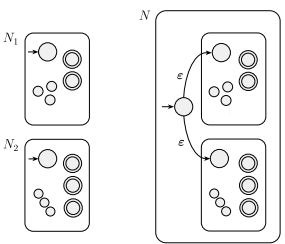
\includegraphics[scale=0.4,right]{Regular_Union.png}
\end{multicols}
\newpage
\begin{multicols}{2}
Concatenation\\
We built a automata M that is the concatenation of $M_1 $ and $M_2$ we simply start with a new start state $M_1$ and for each accept state in $M_1$ we go to the start state of $M_2$ $A_1 \circ A_2$\\
$Q = Q_1 \cup Q_2 $\\
out star state is the same start state as $q_1$ in $M_1$ \\
the accept states $F_2$ are the accept states for $M_2$
our transtion funciton is \\
\[
\delta(q,a) = \left\{
                \begin{array}{ll}
                \delta_1(q,a) 	& q \in Q_1$ and $q \not\in F_1  \\
\delta_1(q,a)  & q \in F_1$ and $ a \neq \epsilon \\
\delta_1(q,a)\cup\{q2\}  & q\in f_1 $ and $ a = \epsilon \\
\delta_2(q,a) & q \in Q_2
\end{array}
\right.
  \]
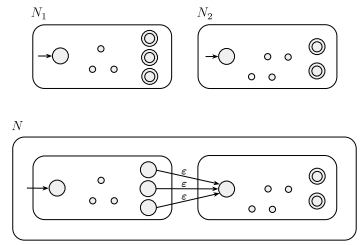
\includegraphics[scale=0.4,right]{Regular_Concatination.png}\\
\end{multicols}
\begin{multicols}{2}
Klein star\\
we need a new state $q_0$ that is also added to F, and we make a transition from all states in F to $q_0$\\

$ Q = q_0 \cup Q$ \\
the state $q_0$ is the new start state.\\
$F = F \cup q_0$ \\
\[
\delta(q,a) = \left\{
 \begin{array}{ll}
\delta_1(q,a) 			 & q \in Q_1$ and $q \not\in F_1  \\
\delta_1(q,a)  			 & q \in F_1$ and $ a \neq \epsilon \\
\delta_1(q,a)\cup\{q_1\} & q\in f_1 $ and $ a = \epsilon \\
\{q_1\}					 & q = q_0$ and $ a = \epsilon \\
\emptyset				 & q = q_0$ and $ a \neq \epsilon \\
\end{array}
\right.
  \]

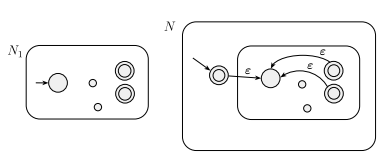
\includegraphics[scale=0.4,right]{Regular_Star.png}\\
\end{multicols}

\subsection{Pumping lemma for regular languages}

The pumping lemma is a way for us to proof if a language is regular. The theorem for the pumping lemma states that the 3 conditions for the lemma is\\
\begin{itemize}
\item for each $i \geq 0, xy^iz \in A $
\item $ |y| > 0 $
\item $ |xy| \leq p$ where p is the pumpking length. 
\end{itemize} 


$0^n1^n | n \geq 0$

The way you do this is to assume it's regular and make a counter argument. with the pumping lemma we have 3 conditions that our counter argument most meet. the first case we can pump the language to have more 1's than 0s or(2) the other way around.. the third(3) is that we can get out of order letters if we pump a string containing both 0s and 1s, 
	


\subsection{Example -> Pumping lemma or convert NFA to DFA}

TODO exam with pumping lemma

\newpage
\section{2. Pushdown automata and context-free languages}


\subsection{Introduction}
I'm going to talk about Pushdown automata and context free languages. These topics are used in compilers to parse a programming language and is a useful tool in language processing as well as when interpreting one language to an other.
\subsection{Pushdown automata}
A pushdown automata is a type of automaton that employs a stack to help with the computation, this allows the PDA to recognize and run Context free grammars as well as the languages within(regular languages).\\

The formal definition is:

\begin{itemize}
\item The set of states Q, 
\item The known alphabet $\Sigma$ (Sigma) 
\item The stack alphabet $\Gamma $ (Gamma)
\item The transition function $\delta (delta): Q \times \Sigma_\epsilon \times \Gamma_\epsilon\longrightarrow Q$
\item the start state $q_0$ 
\item the set of reject states states F
\end{itemize} 
\subsection{Context free grammar}
A CFG consist of a collection of substitution rules, a CFG operate on a set of variables, terminals and a designated start symbol.\\
The formal definition is
\begin{itemize}
\item The finite set of variables V
\item The finite set of terminals $\Sigma$ disjoint from V
\item The finite set of rules R
\item The start symbol $S \in V$
\end{itemize}
\subsubsection{Exsample}
 \begin{multicols}{3}
\begin{itemize}
\item $A \rightarrow 0A1$
\item $A \rightarrow B$
\item $B \rightarrow \# $
\end{itemize}
\end{multicols}
 
This above grammar should generate the string $0^n\#1^n$ $n \in \mathbb{N} $.\\

A different examples that show ambiguity is the set of variables and terminals \{num,A,-\}\\
With the rules\
 \begin{multicols}{3}
\begin{itemize}
\item $A \rightarrow A-A $
\item $A \rightarrow num$
\end{itemize}
\end{multicols}

for the above grammar if we apply it to the string\\
1-2-3 we can get the output 2 or -4 depending on how the grammar is parsed. (1-2)-3 vs 1-(2-3)\\
We can handle this ambiguity in two manners either we introduce the terminals ( and ) to the language or we can rewrite or rules as to not have this issue.\\

\subsection{Chomsky normal Form}
Chomsky normal form is a simplified form that we can convert our grammars into which enables to decide things like if a string is generated by a grammar in polynomial time 2n-1\\

The steps to convert a gramma to CNF is to:\\
\begin{enumerate}
\item eliminate all $\epsilon$ productions.
\item Eliminate all productions where RHS is one variable
\item Eliminate all productions longer than 2 variables
\item move all terminals to productions where RHS is one terminal.
\end{enumerate}
\subsection{Example with CFG -> CNF}

We start in the initial state \\
$ A \rightarrow BAB | B | \epsilon $\\
$ B \rightarrow 00 | \epsilon $ \\
\vspace{5mm}
From here we put a new start state S\\
\vspace{5mm}
$ S \rightarrow A$\\
$ A \rightarrow BAB | B | \epsilon $\\
$ B \rightarrow 00 | \epsilon $\\
\vspace{5mm}
From here we can eliminate the first $\epsilon$ \\
\vspace{5mm}
$ S \rightarrow A$\\
$ A \rightarrow BAB | B | \epsilon \textcolor{OliveGreen}{|BA|AB}$\\
$ B \rightarrow 00 $ $\textcolor{OliveGreen}{\cancel{ | \ \epsilon \ }}$\\

From here we can eliminate the $\epsilon$  in our 2nd rule, \\
\vspace{5mm}
$ S \rightarrow\Ccancel[red]{ | \ A \ |} \textcolor{red}{ BAB|\Ccancel[Cyan]{ B |}BA|AB|\epsilon} \textcolor{Cyan}{|CC}$\\
$ A \rightarrow BAB | \Ccancel[Cyan]{ B |} {\Ccancel[red]{  \ \epsilon \ |}} \textcolor{OliveGreen}{BA|AB} \textcolor{Cyan}{|CC}$\\
$ B \rightarrow \Ccancel[Cyan]{ 00 |}  \Ccancel[OliveGreen]{ \epsilon | } CC$\\
$ \textcolor{Cyan}{C -> 0} $

\subsection{Pumping lemma of non-CFL}
The pumping lemma is a way for us to proof if a language is regular. The theorem for the pumping lemma states that the 3 conditions for the lemma is\\
\begin{itemize}
\item for each $i \geq 0, uv^ixy^iz \in A $
\item $ |vy| > 0 $
\item $ |vxy| \leq p $
\end{itemize}

\subsubsection{Example}
The way you do this is to assume it's regular and make a counter argument. with the pumping lemma we have 3 conditions that our counter argument most meet.\\

$a^nb^nc^n | n \geq 0$

\begin{itemize}
\item if vy only contain the same symbol the string connot contain an equal number of letters as required
\item when either v or y contains more than 1 type of symbol we get an out of order contradiction
\end{itemize}
\newpage
\section{3. Turing machines}

\subsection{Introduction}
In this talk i'll talk about turning machines and their use in computer science, A turning machine is a theoretical form of computer in the same sense as the other models but it's the closets one to modern computers and we can use it for decide things wet. to run time, and compatibility of problems and algorithms.\\

\subsection{What is a turing machine}
    What is a turing machine, The model itself is of a tape and a read/write head that can move left or right on the tape.\\
\begin{itemize}
\item Q is the set of states
\item $\sum$ is the input alphabet not containing the blank symbol $\textvisiblespace$
\item $\tau$ is the tape alphabet where  $\textvisiblespace \in \tau$ and $\sum \subseteq \tau $
\item  $\delta: Q \times \tau \rightarrow Q \times \tau \times \{L,R\} $ is the transition function.
\item $q_0 \in Q$ is the starte states
\item $q_{accept} \in Q$ is the accept state
\item $q_{reject} \in Q $is the reject state where $q_{reject} \neq q_{accept}$ 
\end{itemize}
    

\subsection{Different types of Turing machines}
All turning machines are equal in power, show why.
\subsubsection{Multitape}

The idea is to show that a multitape turing machine $TM_m$ can be simulated on a equivalent single tape turing machine. this is done by storing the tapes on a single tape and discriminating them via the letter $\#$, \\

And we use dot to mark the position of the read head on the underlying tapes. 
If we reach the condition where one of the simulated readheads reaches a $ \# $ symbol on the right side of the simulated tape we write a \textvisiblespace \ and shift the contents of the tape by 1,  
\subsubsection{Nondetermanistic turning machine}
A ND turing machine can be simulated by running a tree search to find accepting state for the desired configuration. and we'll want to approach this in a breath first search as using a dept first can result in following a infinite branch that never reaches a accept state, therefor it's better running a breath first as we're guaranteed to find a accept state should one exist but the issue of looping still exists.

We further call a non deterministic turing machine a decider if all branches halt on all input.

\subsection{Enumerators}

Is a turing machine attached to a printer, basically it generates all possible outputs for a set configuration.

\subsubsection{Theorem 3.21}
A language is only turing recognizable if and only if some enumerator enumerates it.

\subsection{The universal turing machine}
Takes a description and some input w and simulates it, it may accept, reject or halt.\\

You could consider a universal turning machine the closets to a regular computer, except of the sense of the memory. A modern computer may have close to a tarabyte of memory but this still isn't the infinite memory of the turing machines.\\

A universal turning machine is a recognizer but not a decider as i recognizes $A_TM$\\


$A_TM $ Is decidabl


\section{Halting problem}
we have a machine N and input w, we present a machine H that decides if N halts or not.\\
\begin{enumerate}
\item If N halts on input w, accepts
\item if N loops on input w, reject
\end{enumerate}
We then build the machine H+, This new machine has the output modified, the idea is then to feed H+ with itself as as input and as the string.
\begin{enumerate}
\item If H+ with input <H+,H+> halts, we loop.
\item If H+ with input <H+,H+> doesn't halts accept.
\end{enumerate}

\subsection{Proof by contradiction}

Assume that $A_tm$ is decidable, \\
Let H be the tm that decides $A_tm$.\\

\[
H(<M,w>) = \left\{
                \begin{array}{ll}
                Accept, if m accepts w\\
                Reject if m does not accept w or loops.
\end{array}
\right.
  \]
Using H, we can construct a new machine D\\

input to D is a turing machine. and problem that D runs is to check weather a machine would accept if given a input of itself.\\

output, do the opposite of what the input does.\\

Now we try to run D with itself as input.

\[
D(<D>) = \left\{
                \begin{array}{ll}
                Accept, if D does not accepts w\\
                Reject if D accepts
\end{array}
\right.
  \]
  
We then we a paradox.\\



\newpage
\section{4. Decidability}
The problem of Decidability is weather or not we can computer something, and what the limits of computers are. we need to use this to know if a problem is solvable or not with the current computational models we have.

\subsubsection{Example}
$0^n1^n $   $ n \geq 0 $ and $n \in \mathbb{N}$ is not decidable for a DFA/DNA, but it is decidable for a PDA\\
But the grammar $0^n1^n $   $ n \geq 0 $ and $n \in \mathbb{N}$ is not decidable for a PDA, but is decidable by a TM

\subsection{$A_{DFA} $ Is decidable}
The idea for this is to present a tm that simulates $A_{DFA}$\\
We build a TM M that takes input <B,w> where B is the DFA and w in our input.\\
1. M first determines if proprerly reprecents a DFA B and the string w, if not it rejects. \\
2. M then simulates B directly keeping track of how much input we have processed and what state we are in, \\
3. When M is done simulating eg, when we reach the end of w we accept if B accepts and rejects if we're in a non-accepting states\\
\subsection{$A_{NFA}$ is decidable}

This can be proven by using the above example as a subroutine, and building make a TM N that first converts $A_{NFA}$ to  a DFA and then run the above problem on it.\\

NFA to DFA theorem chapter 1 theorem 39

\subsection{$A_{REX}$ is decidable}

a regex can be converted into a NFA (theorem 1.54)

We present a turing machine that P that converts the regex into a NFA, we can then run N as a subroutine and show that RegEX is decidable.

\subsection{$A_{CFG}$ is decidable}
we build a TM S, we take input <G,w> where G is a CFG and w is a string\\

\begin{enumerate}
\item convert G into Chomsky normal form.
\item list all derivations with 2n-1 steps,  where n in the length of the string, except the case where n in length zero when then list all derivations with 1 step.\
\item if any of these derivations generate w accept else reject.\\
\end{enumerate}

This same tm can be used to show that all Context free languages are decidable\

\subsection{undecidability}
Some problems are also undecidable, for example Uncountability, and not all turning machines are decidable.
\subsection{countability and Uncountability}
some finite sets we can simply count them, but how can we prove that one infinite set in larger than an other.\\
We use the following definition of countable, if our set has a finite size, or if there is a correspondence with $\mathbb{N}$\\

\subsubsection{The set of odd numbers}

The correspondence with off numbers is that we can simply map f(n) = 2n-1, where n is our regular numbers. here our odd numbers are also a subset of our natural numbers

\subsection{The set of rational numbers}

rational numbers can be expressed as $\{\frac{m}{n} | m $ and $ n \in \mathbb{N}$\\

This set of countable infinite. this can by shown by using the The diagonalization method

The way that we can generate a list of all rational numbers. is to go over a matrix 

\newcounter{nodecount}
% Command for making a new node and naming it according to the nodecount counter
\newcommand\tabnode[1]{\addtocounter{nodecount}{1} \tikz \node (\arabic{nodecount}) {#1};}


\begin{table}[h]
\begin{tabular}{cccccc}
\diagbox{M}{N}& 1 & 2 & 3 & 4 & ... \\
1                  & \tabnode{\circled{$\frac{1}{1}$}}  & \tabnode{\circled{$\frac{1}{2}$}}  & \tabnode{\circled{$\frac{1}{3}$}}  & \tabnode{\circled{$\frac{1}{4}$}} & ...  \\
2                  & \tabnode{\circled{$\frac{2}{1}$}}  & $\cancel{\frac{2}{2}}$   & \circled{$\frac{2}{3}$}  & $\cancel{\frac{2}{4}}$  & ... \\
3                  & \tabnode{\circled{$\frac{3}{1}$}}  & \circled{$\frac{3}{2}$}  & $\cancel{\frac{3}{3}}$   & $\cancel{\frac{3}{4}}$ & ... \\
4                  & \tabnode{\circled{$\frac{4}{1}$}}  & $\cancel{\frac{4}{2}}$   & $\cancel{\frac{4}{3}}$   & $\cancel{\frac{4}{4}}$ & ... \\
... & ... & ... & ... & ... & ...
\end{tabular}

\begin{tikzpicture}[overlay]
% Define the circle paths

\end{tikzpicture}

\end{table}

\subsection{Irrational numbers}

The set of irrational numbers is a uncountable infinite set. numbers like $\pi, \sqrt{2}, e$ and so on have a infinite numbers of digits.\\
between two ration numbers we have a infinite irrational numbers.\\

Proof by contradiction. assume that the set $\mathbb{I}$ is countable infinite.\\

this can be shown via:
\subsection{The diagonalization method.}
we can build a new number, that can't be in the table, which gives us a contradiction in the table.


\section*{some langues are not turing recognizable}
We can show that we have a countable infinite amount of turing machines.
\begin{itemize}
\item every turing machine can be coded into a string, that have a finite length
\item everything is either a valid turing machine or "garbage"
\item Generate one string after the other
\item check to see if it is a valid turing machine.
\end{itemize}
\subsubsection{Proof (By diagonalization method)} 

We can show that there are uncountable infinite many strings.\\
We can show that we have a uncountable infinite amount of infinte strings over \{0,1\}\\

same idea as $\mathbb{I}$ uncountability, by flipping the bit. this we we can generate a new string that is infinite length and that is not in the table.\\

therefor: The number of languages is countably infinite.\\

and by the first example we showed that the set of all turing machines is countably infinite, and from this we have the corollary that the set of all turing-recognizable languages is countably infinite.\\
and we showed that the set of all langues is countably infinite.\\
We therefor have the corollary that some languages are not turing recognizable\\

\subsection{A language that isn't turing recognizable}

If a language L is decidable, then L is turing recognizable, and it's complement $\overline{L}$ is turing recognizable\\
\begin{itemize}
\item Every decidable language is turing recognizable
\item want to recognize $\overline{L}$ just run the decider for L and give the opposite answer.
\end{itemize}

We run the machine for L and $\overline{L}$ in parallel. eg running one step on each until one of them reaches a accept state, and one of them has to be in one of them. and one or both of them has to halt.\\

If that machine for L accepts we accept, and if the machine for it's complement $\overline{L}$ accepts we reject. either way we'll always halt\\

with this it can be shown, that a language is only decidable if both it and it's complement are turing recognizable. \\

a language is co-turing recognizable is if it's complement is turning recognizable \\

we know that $A_{TM}$ is turning recognizable,\\
and that $A_{TM}$ is not decidable\\

Therefor $\overline{A_{TM}}$ is not turing recognizable

We can proof this as $A_{TM}$ is not decidable.
 
\newpage
\section{5. Reducibility}

\subsection{Introduction}

Reduciblity is the method of proving by mapping a more complex problem to a simpler one, and by this we can proof that if a problem is decidable or not. You must however be very careful when doing this at it can only be done if the problems are the same in nature.\\
The first thing we need to do when we are preforming this method is to have a problem that we can reduce to, This problem has to be mappable to our simpler problem and the property we want to map to has to be shown to be undecidable, in this case the $A_TM$ problem will be used, the problem for $A_TM$ is solved via the diagonalization method.
\subsubsection{Reduction to halting problem} 
With $A_{TM}$ we can show that $halt_{TM}$ is undecidable.





\newpage
\section{6. NP-completeness proofs – examples.}
what is np\_completeness

Why we use it to reduce,

Proff of np complete.
qlique, 

subset sum, 

Hamiltonian circuit, 






\newpage
\section{7. Proof that SATISFIABILITY is NP-complete (do not assume that
there is a known NP-Complete problem — use the proof in Sipser’s
book).}

Cook-levin theorem - in sipset, presentation use slides on homepage.


\newpage
\section{8. Information-theoretic lower bounds}

(lower bounds proven by counting leaves in decision trees), especially the average case bounds for sorting
by comparisons.

As is average case.




\newpage
\section{9. Adversary arguments – technique, examples.}





\newpage
\section{10. Median problem – algorithm and lower bound.}





\newpage
\section{11. Approximation algorithms}

vertex cover



\chapter{Exercises 2019}

\section{Week 1}

\subsection{page 84, question 1.7}

\subsubsection{a}

{w|w begins with a 1 and ends with a 0} \\
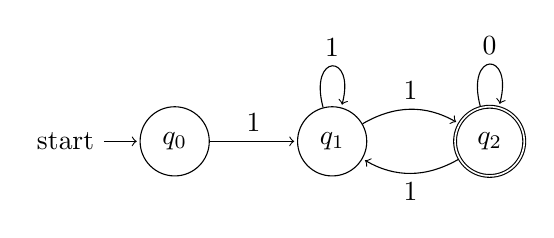
\begin{tikzpicture}[shorten >=1pt,node distance=2cm,on grid,auto] 
   \node[state,initial] (q_2)   {$q_0$}; 
   \node[state] (q_0)  [right=of q_2] {$q_1$}; 
   \node[state,accepting](q_1) [right=of q_0] {$q_2$};
    \path[->] 
    (q_0) edge [bend left]node {1} (q_1)
          edge [loop above] node {1} (q_0)
    (q_1) edge [bend left]node  {1} (q_0)
          edge [loop above] node {0} ()
    (q_2) edge node {1} (q_0);
\end{tikzpicture}


\subsubsection{b}
{w|w contains at least 3 1's}\\
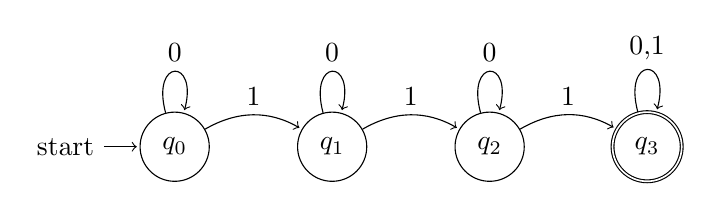
\begin{tikzpicture}[shorten >=1pt,node distance=2cm,on grid,auto] 
   \node[state,initial] (q_0)   {$q_0$}; 
   \node[state](q_1) [right=of q_0] {$q_1$};
   \node[state](q_2) [right=of q_1] {$q_2$};
   \node[state,accepting](q_3) [right=of q_2] {$q_3$};
    \path[->] 
    (q_0) edge [bend left]node {1} (q_1)
          edge [loop above] node {0} ()
    (q_1) edge [bend left]node  {1} (q_2)
          edge [loop above] node {0} ()
    (q_2) edge [bend left]node  {1} (q_3)
          edge [loop above] node {0} ()
    (q_3) edge [loop above] node {0,1} ();
\end{tikzpicture}


\subsubsection{c}
{w|w contains the substring 0101, (i.e. w = x0101y for some x and y)}
\\
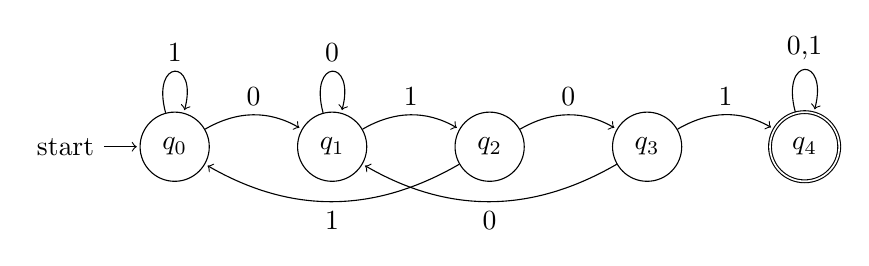
\begin{tikzpicture}[shorten >=1pt,node distance=2cm,on grid,auto] 
   \node[state,initial] (q_0)   {$q_0$}; 
   \node[state](q_1) [right=of q_0] {$q_1$};
   \node[state](q_2) [right=of q_1] {$q_2$};
   \node[state](q_3) [right=of q_2] {$q_3$};
      \node[state,accepting](q_4) [right=of q_3] {$q_4$};
    \path[->] 
    (q_0) edge [bend left]node {0} (q_1)
          edge [loop above] node {1} ()
          
    (q_1) edge [bend left]node  {1} (q_2)
          edge [loop above] node {0} ()
          
    (q_2) edge [bend left]node  {0} (q_3)
          edge [bend left] node {1} (q_0)
          
    (q_3) edge [bend left]node  {1} (q_4)
          edge [bend left] node {0} (q_1)
          
    (q_4) edge [loop above] node {0,1} ();
\end{tikzpicture}

\subsubsection{d}
{w|w bas at length of at least 3 and it's third symbol is 0}
\\
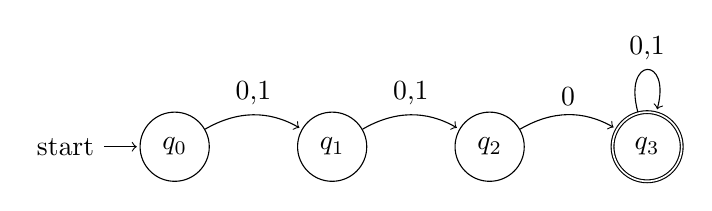
\begin{tikzpicture}[shorten >=1pt,node distance=2cm,on grid,auto] 
   \node[state,initial] (q_0)   {$q_0$}; 
   \node[state](q_1) [right=of q_0] {$q_1$};
   \node[state](q_2) [right=of q_1] {$q_2$};
   \node[state,accepting](q_3) [right=of q_2] {$q_3$};
    \path[->] 
    (q_0) edge [bend left]node {0,1} (q_1)
    (q_1) edge [bend left]node  {0,1} (q_2)
    (q_2) edge [bend left]node  {0} (q_3)
    (q_3) edge [loop above] node {0,1} ();
\end{tikzpicture}

\subsubsection{f}
{w|w doesn't contain the substring 001} \\
Accepts any string that doesn't contain the substring 001, and loops in rejecting state if this state is found, was unsure if the looping was needed but included it if it was the case.\\
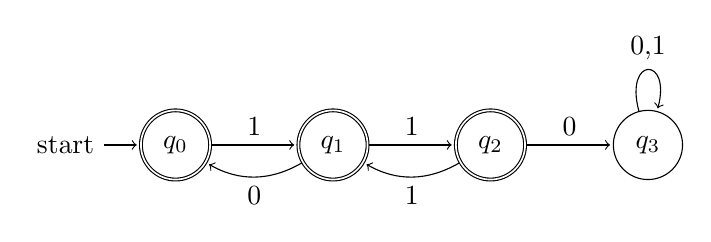
\begin{tikzpicture}[shorten >=1pt,node distance=2cm,on grid,auto] 
   \node[state,initial,accepting] (q_0)   {$q_0$}; 
   \node[state,accepting](q_1) [right=of q_0] {$q_1$};
   \node[state,accepting](q_2) [right=of q_1] {$q_2$};
   \node[state](q_3) [right=of q_2] {$q_3$};
    \path[->] 
    (q_0) edge node {1} (q_1)
    (q_1) edge node  {1} (q_2)
          edge [bend left] node {0} (q_0)
    (q_2) edge node  {0} (q_3)
    	edge [bend left] node {1} (q_1)
    (q_3) edge [loop above] node {0,1} ();
\end{tikzpicture}
\\

\subsubsection{h}
{w|w is any string except 11 and 111}\\
accepts any string that isn't 11, 111 including the empty string $\epsilon $ \\
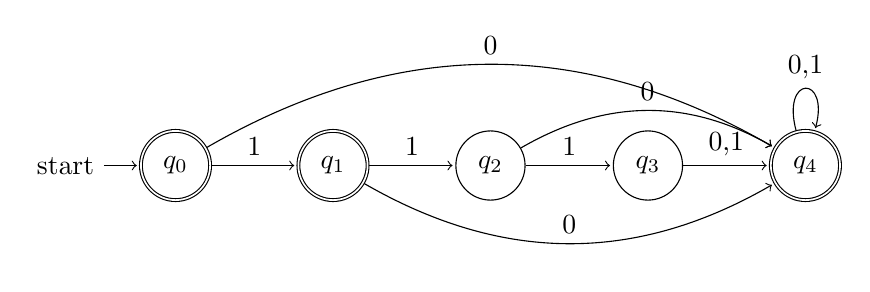
\begin{tikzpicture}[shorten >=1pt,node distance=2cm,on grid,auto] 
   \node[state,initial,accepting] (q_0)   {$q_0$}; 
   \node[state,accepting](q_1) [right=of q_0] {$q_1$};
   \node[state](q_2) [right=of q_1] {$q_2$};
   \node[state](q_3) [right=of q_2] {$q_3$};
   \node[state,accepting](q_4) [right=of q_3] {$q_4$};
    \path[->] 
    (q_0) edge node {1} (q_1)
   		  edge [bend left] node {0} (q_4)
    (q_1) edge node  {1} (q_2)
    	  edge [bend right] node {0} (q_4)
    (q_2) edge node  {1} (q_3)
    	  edge [bend left] node {0} (q_4)
    (q_3) edge node {0,1} (q_4)
    (q_4) edge [loop above] node {0,1} ();
\end{tikzpicture}

\subsubsection{i}
{w|w every odd position of w is a 1} \\
accepts all states where \#1\#1\#1\#1\#1 is followed also accepts the empty string $ \epsilon $ \\


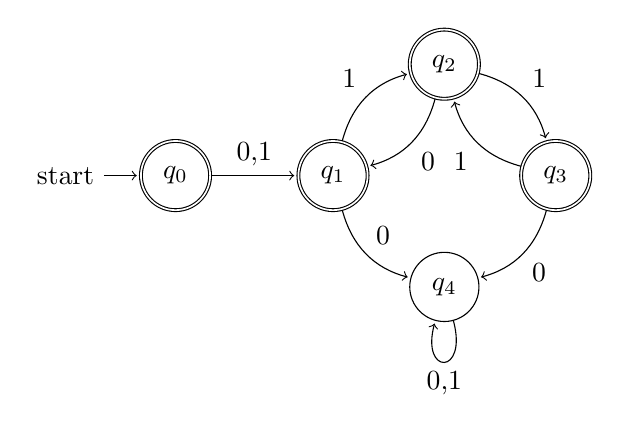
\begin{tikzpicture}[shorten >=1pt,node distance=2cm,on grid,auto] 
   \node[state,initial,accepting] (q_0)   {$q_0$}; 
   \node[state,accepting](q_1) [right=of q_0] {$q_1$};
   \node[state,accepting](q_2) [above right=of q_1] {$q_2$};
   \node[state](q_4) [below right=of q_1] {$q_4$};
   \node[state,accepting](q_3) [above right=of q_4] {$q_3$};
    \path[->] 
    (q_0) edge node {0,1} (q_1)
    (q_1) edge [bend left]node  {1} (q_2)
          edge [bend right] node {0} (q_4)
    (q_2) edge [bend left] node  {1} (q_3)
    	  edge [bend left] node {0} (q_1)
    (q_3) edge [bend left] node {0} (q_4)
   		  edge [bend left] node {1} (q_2)
   	(q_4) edge [loop below] node {0,1} ();
\end{tikzpicture}


\subsubsection{k}
{w|w is only the empty string and 0} \\
accepts "0" and the empty string $ \epsilon $ \\


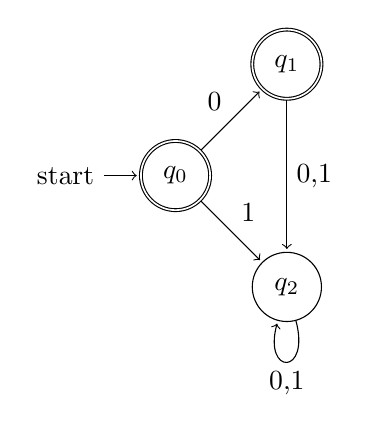
\begin{tikzpicture}[shorten >=1pt,node distance=2cm,on grid,auto] 
   \node[state,initial,accepting] (q_0)   {$q_0$}; 
   \node[state,accepting](q_1) [above right =of q_0] {$q_1$};
   \node[state](q_2) [below right =of q_0] {$q_2$};

    \path[->] 
    (q_0) edge node {0} (q_1)
    	  edge node  {1} (q_2)
    (q_1) edge node {0,1} (q_2)
   	(q_2) edge [loop below] node {0,1} ();
\end{tikzpicture}

\newpage
\subsection{page 84, question 1.7}

\subsubsection{d}
The language {0} with two states,\\

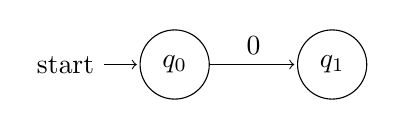
\begin{tikzpicture}[shorten >=1pt,node distance=2cm,on grid,auto] 
   \node[state,initial] (q_0)   {$q_0$}; 
   \node[state](q_1) [right =of q_0] {$q_1$};

    \path[->] 
    (q_0) edge node {0} (q_1);
\end{tikzpicture}
\subsubsection{e}
the language 0*1*0* with 3 states \\
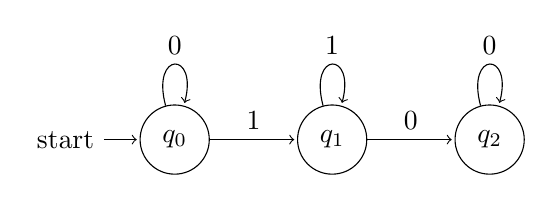
\begin{tikzpicture}[shorten >=1pt,node distance=2cm,on grid,auto] 
   \node[state,initial] (q_0)   {$q_0$}; 
   \node[state](q_1) [right =of q_0] {$q_1$};
   \node[state](q_2) [right =of q_1] {$q_2$};

    \path[->] 
    (q_0) edge node {1} (q_1)
    	edge [loop above]node  {0} (q_2)
    (q_1) edge node {0} (q_2)
    edge [loop above]node  {1} (q_2)
   	(q_2) edge [loop above]node  {0} (q_2);
\end{tikzpicture}
\subsubsection{g}
the language {$\epsilon$} with 1 state \\

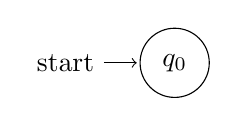
\begin{tikzpicture}[shorten >=1pt,node distance=2cm,on grid,auto] 
   \node[state,initial] (q_0)   {$q_0$}; 
\end{tikzpicture}


\subsubsection{h}
The language 0* with 1 state \\

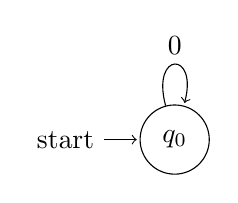
\begin{tikzpicture}[shorten >=1pt,node distance=2cm,on grid,auto] 
   \node[state,initial] (q_0)   {$q_0$}; ;

    \path[->] 
    (q_0) [loop above]edge node {0} ();
\end{tikzpicture}


\subsection{Solve the following problem,}

A man is travelling with a wolf (w) and a goat (g). He also brings along a nice big
cabbage (c). He encounters a small river which he must cross to continue his travel.
Fortunately, there is a small boat at the shore which he can use. However, the boat
is so small that the man cannot bring more than himself and exactly one more item
along (from {w, g, c}). The man knows that if left alone with the goat, the wolf will
surely eat it and the goat if left alone with the cabbage will also surely eat that. The
man’s task is hence to device a transportation scheme in which, at any time, at most
one item from {w, g, c} is in the boat and the result is that they all crossed the river
and can continue unharmed.

\subsubsection{a} Describe a solution to the problem which satisfies the rules of the “game”. You may use your answer to (b) to find a solution. \\

\begin{itemize}
\item First you carry the goat to the other side, and go back empty.
\item The you ferry the wolf to the other side, and swap with the goat and bring the goat back.
\item you then swap the goat with the cabbage and bring it to the other side.
\item lastly you head back empty and bring the goat.
\item you now have all the items on the other side of the river.
\end{itemize}


\subsubsection{b}
The string all of the valid moves are 
\begin{equation}
\begin{split}
(g(m(x(g(y(m(g)*)*)*)*)*)*)* \\
x,y = (w|c) \\
x \neq y
\end{split}
\end{equation}


\vspace{5mm}
This is due to the fact that it's legal moves in the game, like the man can bring the goat to the other side and bring it back too, it's bad move, but it's still a valid move. \\

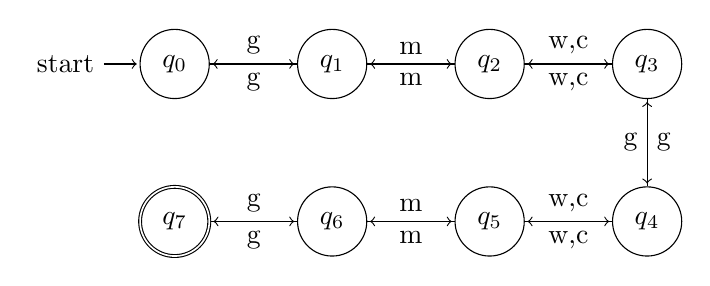
\begin{tikzpicture}[shorten >=1pt,node distance=2cm,on grid,auto] 
   \node[state,initial] (q_0)   {$q_0$}; 
   \node[state](q_1) [right =of q_0] {$q_1$};
   \node[state](q_2) [right =of q_1] {$q_2$};
   \node[state](q_3) [right =of q_2] {$q_3$};
   \node[state](q_4) [below =of q_3] {$q_4$};
   \node[state](q_5) [left =of q_4] {$q_5$};
   \node[state](q_6) [left =of q_5] {$q_6$};
   \node[state,accepting](q_7) [left =of q_6] {$q_7$};

    \path[->] 
    (q_0) edge node {g} (q_1)
    (q_1) edge node {g} (q_0)
   	      edge node {m} (q_2)
    (q_2) edge node {m} (q_1)
   	      edge node {w,c} (q_3)
   	(q_3) edge node {w,c} (q_2)
   	      edge node {g} (q_4)
   	(q_4) edge node {g} (q_3)
   	      edge node {w,c} (q_5)
   	(q_5) edge node {w,c} (q_4)
   	      edge node {m} (q_6)
   	(q_6) edge node {m} (q_5)
   	      edge node {g} (q_7)   	      
   	(q_7) edge node {g} (q_6);
\end{tikzpicture}




\section{Week 2}

\subsection{page 86, question 1.16}
* is zero or more \\
! is one or more \\

\subsubsection{a}
it accepts (bb)*a!(a|b)* \\

the language 0*1*0* with 3 states \\
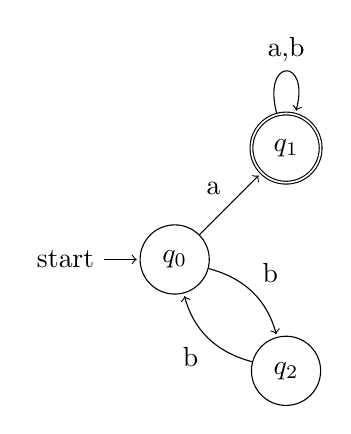
\begin{tikzpicture}[shorten >=1pt,node distance=2cm,on grid,auto] 
   \node[state,initial] (q_0)   {$q_0$}; 
   \node[state,accepting](q_1) [above right =of q_0] {$q_1$};
   \node[state](q_2) [below right =of q_0] {$q_2$};

    \path[->] 
    (q_0) edge node {a} (q_1)
   		  edge [bend left]node {b} (q_2)
    (q_1) edge [loop above]node {a,b} (q_1)
   	(q_2) edge [bend left]node  {b} (q_0);
\end{tikzpicture}

\subsubsection{b}


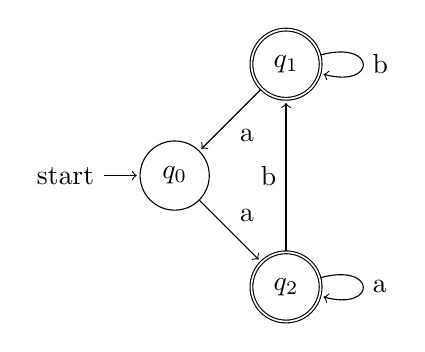
\begin{tikzpicture}[shorten >=1pt,node distance=2cm,on grid,auto] 
   \node[state,initial] (q_0)   {$q_0$}; 
   \node[state,accepting](q_1) [above right =of q_0] {$q_1$};
   \node[state,accepting](q_2) [below right =of q_0] {$q_2$};

    \path[->] 
    (q_0) edge node {a} (q_2)
   		  
    (q_1) edge node {a} (q_0)
    	  edge [loop right]node {b} ()
   	(q_2) edge [loop right]node  {a} ()
   	      edge []node  {b} (q_1);
\end{tikzpicture}

\subsection{page 86, question 1.17}

\subsubsection{a}
The first task is to make a NFA recognizing (01u001u010)* \\
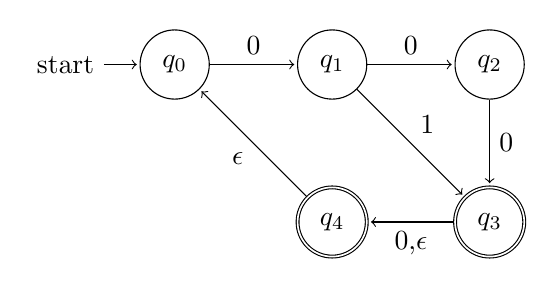
\begin{tikzpicture}[shorten >=1pt,node distance=2cm,on grid,auto] 
   \node[state,initial] (q_0)   {$q_0$}; 
   \node[state](q_1) [right =of q_0] {$q_1$};
   \node[state](q_2) [right =of q_1] {$q_2$};
   \node[state,accepting](q_3) [below =of q_2] {$q_3$};
   \node[state,accepting](q_4) [below =of q_1] {$q_4$};



    \path[->] 
    (q_0) edge node {0} (q_1)
    (q_1) edge node {0} (q_2)
    	  edge node {1} (q_3)
   	(q_2) edge node {0} (q_3)
   	(q_3) edge node {0,$\epsilon$} (q_4)
   	(q_4) edge node {$\epsilon$} (q_0);
\end{tikzpicture}
\\

\subsubsection{b}
After converting this to a DFA\\

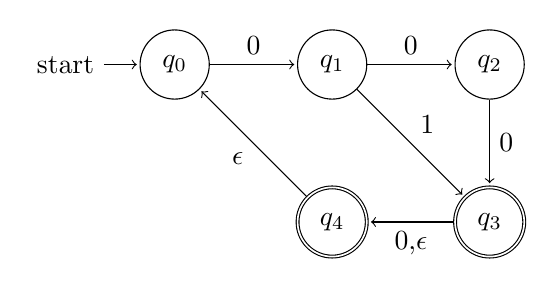
\begin{tikzpicture}[shorten >=1pt,node distance=2cm,on grid,auto] 
   \node[state,initial] (q_0)   {$q_0$}; 
   \node[state](q_1) [right =of q_0] {$q_1$};
   \node[state](q_2) [right =of q_1] {$q_2$};
   \node[state,accepting](q_3) [below =of q_2] {$q_3$};
   \node[state,accepting](q_4) [below =of q_1] {$q_4$};



    \path[->] 
    (q_0) edge node {0} (q_1)
    (q_1) edge node {0} (q_2)
    	  edge node {1} (q_3)
   	(q_2) edge node {0} (q_3)
   	(q_3) edge node {0,$\epsilon$} (q_4)
   	(q_4) edge node {$\epsilon$} (q_0);
\end{tikzpicture}

\subsection{page 86, question 1.18}
Predefined terms
\begin{equation}
x = (0,1)^*
\end{equation}
\begin{equation}
y = (0|1)
\end{equation}

\subsubsection{a}
$1x0$
\subsubsection{b}
$x1x1x1x$
\subsubsection{c}
$x0101x$
\subsubsection{d}
$yy0x$
\subsubsection{e}
$(0(yy)*)|1y(yy)^*)$
\subsubsection{f}
$ 0^*(1+10)^* $
\subsubsection{g}
$ yyyyy $


\subsection{page 86, question 1.19 a}

Convert the following regex to a NFA via lemma 1.55\\
\begin{equation}
(0 \cup 1)^*000(0\cup 1)^* 
\end{equation}
\begin{center}


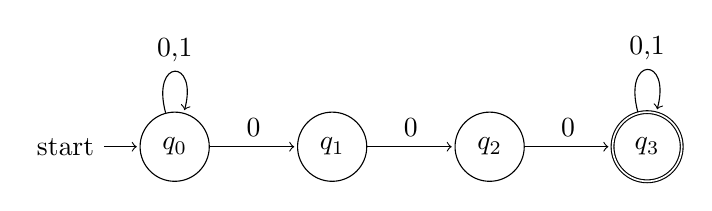
\begin{tikzpicture}[shorten >=1pt,node distance=2cm,on grid,auto] 
   \node[state,initial] (q_0)   {$q_0$}; 
   \node[state](q_1) [right =of q_0] {$q_1$};
   \node[state](q_2) [right =of q_1] {$q_2$};
   \node[state,accepting](q_3) [right =of q_2] {$q_3$};



    \path[->] 
    (q_0) edge [loop above] node {0,1} (q_0)
    	  edge node {0} (q_1)
    (q_1) edge node {0} (q_2)
   	(q_2) edge node {0} (q_3)
   	(q_3) edge [loop above] node {0,1} ();
\end{tikzpicture}
\end{center}

\subsection{page 86, question 1.20}
For each of the following expressions give two strings that are and two that are not in the languages. assume that the alphabet is \{a,b\}
\begin{multicols}{2}
\subsubsection{a}
\begin{equation}
a^*b^*
\end{equation}
member\\
aa, ab, aabb, aab, abbbb\\
not member\\
ba, abab, \\
\subsubsection{b}
\begin{equation}
a(ba)^*b
\end{equation}
member\\
abab, ababababab,\\
not member\\
aaba baba\\
\subsubsection{c}
\begin{equation}
a^* \cup B^*
\end{equation}
member\\
ab, aabb \\
not member \\
ba, aabba\\
\subsubsection{d}
\begin{equation}
(aaa)^*
\end{equation}
member\\
aaa, aaaaaa \\
not member\\
a, aaaa\\
\subsubsection{e}
\begin{equation}
\sum^*a\sum^*b\sum^*a\sum^*
\end{equation}
member\\
todo\\
not member\\
todo\\
\subsubsection{f}
\begin{equation}
aba \cup bab
\end{equation}
member \\
todo\\
not member\\
todo\\
\subsubsection{g}
\begin{equation}
(\epsilon \cup a)b
\end{equation}
member\\
ab, b\\
not member\\
abb, aab\\
\subsubsection{h}
\begin{equation}
(a\cup ba \cup bb)\sum^*
\end{equation}
member\\
todo\\
not member\\
todo \\
\end{multicols}
\subsection{page 86, question 1.21 b}

The solution is 
\begin{equation}
((a|b)(a,bb)*b(a)?)*
\end{equation}
(a or b, followed by any number of (a,bb)* followed by a single b (as it matches uneven numbers of b and followed by 0 or 1 a*

\subsection{page 86, question 1.29}

\subsubsection{a}

For the task a we have the sting 
\begin{equation}
0^n1^n2^n
\end{equation}
the first contradiction is that when we have a string eg. 000111222 and we split it so we have the floowing, x = 000, y = 111, z = 222 and we pump y so we have the string xyyz this violates the first condition of the pumping lemma, as we'll have more 1s then 0s and 2s.

the string y only contains 1s which also causes a contradiction.

and the 3rd case if we have the string x = 00, y = 011 and z = 1222 where we'll get out of order letters so we'll again reach a contradiction.


\subsubsection{b}

For assignment b i find it a bit odd, i may misunderstand the exercise but w/e

We want to pump the language
\begin{equation}
a_2 = \{www|w \in \{a,b\}^*\}
\end{equation}
But from my understanding is the * a kleen star? eg then one w and www are equivalent as \{a,b\} is all possibly strings in the library w. ? or is it understand such that w is equal to either a or b but any number of them eq $\{a|b\}^*$,\\
How i choose to intercept it for now is that w is equal to either the string a* or b* and if this is the case then some of the same argumentation as for task a is valid.
\\
www can give us the string 111000111 and we can split it as follows. 111|1000|11111, This means that zyyx gives of a out of order 1 and we therefor get a contradiction wrt. to the pumping lemma.


\subsection{page 88, question 1.30}
The error There's a few things here, the first case from 1:73 fail right away as the string 0001111 is in the lang, the case of out of order fails as if we can get the string 00100111 ten we'll reach a contradiction but the case of 



\subsection{page 89, question 1.36}

For the language w there exist a DFA that accepts if, for the revere language $w^r$ the DFA which a reversed edges and the start state is now our accept state. 


\section{week 3}

\subsection{page 88, question 1.29(a),(b) and 1.30}

Already done, see above.

\subsection{page 89. question 1.35}
As B is in bijection of A therefor it's a regular.


\subsection{page 91. question 1.51}
\begin{multicols}{2}


\subsubsection{a}
This can be proved via the pumping lemma. where you can get out of order 1 and/or 0s and that causes a contradiction.

\subsubsection{b}
Same as a wrt. our of order.

\subsubsection{c}

This is this is either the unbounded string 0 or 1.

\subsubsection{d}
this is again wrt. out of order 0.1 eg. if we can get the string 01010 by umping as this is not in the lang.
\end{multicols}
\subsection{page 154. question 2.2}
Give parse trees and derivations for each string using the following Context free gramma (CFG)  \\
\begin{center}
$ E \rightarrow E+T | T$ \\
$ T \rightarrow E \times F | F $ \\
$ F \rightarrow (E) | a$
\end{center}


\begin{figure}[h]%
    \centering
    \subfloat[a]{{\Tree[.E [.T [.F [a ]]]] }}%
    \qquad
    \subfloat[a+a]{{\Tree
	[.E 
		[.T [.F [a ]]]
		+
		[.E [.T [.F [a ]]]]
	] }}%
	\qquad
    \subfloat[a+a+a]{{
    \Tree
	[.E 
		[.T [.F [a ]]]
		+
		[.E [.T [.F [a ]]]
			+
			[.E [.T [.F [a ]]]		
		]
	]]
	}}%
	    \subfloat[((a))]{{
	\Tree
	[.E 
		[.T [.F [( [.E [.T [.F [( [[.T [.F [a ]]]] ) ]]]] ) ]]]
	]
	}}%
    \caption{2 Figures side by side}%
    \label{fig:example}%
\end{figure}

\subsection{page 154. question 2.4}
\begin{multicols}{2}
\subsubsection{a}
$ S \rightarrow TTT $\\
$ T \rightarrow E1E $\\
$ E \rightarrow FTF $\\
$ F \rightarrow 0 | \epsilon $\\
\subsubsection{b}
$ S \rightarrow 0F0 | 1F1 $\\
$ F \rightarrow F0F | F1F | \epsilon $\\
\subsubsection{c}
$ S \rightarrow EFE $\\
$ E \rightarrow FEF | EFF | FFE | \epsilon $\\
$ F \rightarrow 0 | 1$
\subsubsection{d}
$ S \rightarrow E0E $\\
$ E \rightarrow FEF | \epsilon $\\
$ F \rightarrow 0 | 1$
\subsubsection{e}
$ S \rightarrow E $\\
$ E \rightarrow FEF | GEG | \epsilon $\\
$ F \rightarrow 0 $
$ G \rightarrow 1 $
\subsubsection{f}
$ S \rightarrow \epsilon $ \\


\end{multicols}
\newpage
\subsection{2.6}
Give the CFG that generates the following languages
\begin{multicols}{2}

\subsubsection{b}
The complment of the langauges $ \{a^nb^n | n \geq 0 \} $

$ S \rightarrow FG $\\
$ G \rightarrow GbG $\\
$ F \rightarrow FaF $

\subsection{d}
For the third one it's a unbounded string with up to k alternations of $0^*1^*0^*1^*0^*$

This can simply be defined using the following grammar.

$ S \rightarrow FG $\\
$ E \rightarrow GE | FE | \epsilon $\\
$ G \rightarrow 1G | \epsilon $\\
$ F \rightarrow 0F | \epsilon $

\end{multicols}


\subsection{2.14}
We start in the initial state \\
$ A \rightarrow BAB | B | \epsilon $\\
$ B \rightarrow 00 | \epsilon $ \\
\vspace{5mm}
From here we put a new start state S\\
\vspace{5mm}
$ S \rightarrow A$\\
$ A \rightarrow BAB | B | \epsilon $\\
$ B \rightarrow 00 | \epsilon $\\
\vspace{5mm}
From here we can eliminate the first $\epsilon$ \\
\vspace{5mm}
$ S \rightarrow A$\\
$ A \rightarrow BAB | B | \epsilon \textcolor{OliveGreen}{|BA|AB}$\\
$ B \rightarrow 00 $ $\textcolor{OliveGreen}{\cancel{ | \ \epsilon \ }}$\\

From here we can eliminate the $\epsilon$  in our 2nd rule, \\
\vspace{5mm}
$ S \rightarrow\Ccancel[red]{ | \ A \ |} \textcolor{red}{ BAB|\Ccancel[Cyan]{ B |}BA|AB|\epsilon} \textcolor{Cyan}{|CC}$\\
$ A \rightarrow BAB | \Ccancel[Cyan]{ B |} {\Ccancel[red]{  \ \epsilon \ |}} \textcolor{OliveGreen}{BA|AB} \textcolor{Cyan}{|CC}$\\
$ B \rightarrow \Ccancel[Cyan]{ 00 |}  \Ccancel[OliveGreen]{ \epsilon | } CC$\\
$ \textcolor{Cyan}{C -> 0} $
\subsection{page 156, question 2.16}
Show that the class of context free languages are closed under the regular operations Concatenation, union and Star\\ 
Using the following grammar \\
\begin{itemize}
\item $ S_1 \rightarrow aS_1b$
\item $ S_1 \rightarrow \epsilon$

\item $ S_2 \rightarrow cS_2d$
\item $ S_2 \rightarrow \epsilon$
\end{itemize}
\subsubsection{Concatenation}
This is simply shown via 

Making s start symbol S, and have the two languages follow each other $S_1$ $S_2$ \\
$S \rightarrow S_1S_2$
\subsubsection{Union}
This is simply shown via 

Making s start symbol S, \\
$S \rightarrow S_1 | S_2$
\subsubsection{Star}
This is simply shown via 

Making s start symbol S, \\
$S \rightarrow S_1S$


\subsection{page 158, question 2.32}
 Let $A/B=\{w|wx \in A$ for some $x \in B \}$, Show that if A is context free and B is regular, then A/B is context free.
 
 "Proof. We can augment the memory of the PDA recognizing the CFL with the DFA recognizing the regular langauge and run both machines in parallel. We accept iff both machines accept.\ref{http://web.mit.edu/bmhuang/www/notes/18404-notes.pdf page 14, 4.3}\\
 note the intersection of two CFL's and not necessarily a CFL.!
 
 
 \subsection{page 158, question 2.38}
 As each step has a most 2 sub rules we can calculate that at step 1 we increasing the string length by 2n-1 and as all rules do this our end case is 2n-1
 
 \subsection{page 158, question 2.42}
 • 2.42 Hint for (d): first intersect the language with a suitably chosen regular language
and then prove that the language you obtain is not context-free.

 \begin{multicols}{2}
\subsubsection{a}
A break wrt. out of order letters, and not n counts of some letter
\subsubsection{b}
For the lang b is has to be in the size of wrt. $n+n^2+n^3$ eg 3,14, 39, 84, 155 and you can pump it to a length not in this range,

\subsubsection{c}
i dont know
\subsubsection{d}
i dont know

\end{multicols}
\newpage
\section{week 4}

\subsection{2.58}

let $\sum = \{0,1\}$ and let B be the collection of strings that contain at least one 1 in their second half, in other words,$ B = \{uv | u \in \sum ^*, v \in \sum^* 1 \sum^*$ and $ |u| \geq |v|\}$
\\
\subsubsection{a}
 Give a PDA that recognizes B
 
$ S \rightarrow XTX | X1$ \\
$ T \rightarrow XT | X $ \\
$ X \rightarrow 1|0$ \\
 
 
 \subsubsection{b}
Give a CFG that generates B
Read the input from end to front, pushing every 0 you meet onto the stack. if a 1 is found you continue parsing but instead pop a letter from the stack until it's empty, if you reach the beginning of the input before the stack is empty you reject.

\subsection{2002 program 2}
Let $\sum$ be a finite alphabet and let $L \subset \sum^+ $ be a regular language, Define a new language L'as the language of all words w $\in \sum^*$ such that w is obtained from a word in L by deleting the first letter, is the language L' regular as well? prove your answer\\





\newpage

 
\end{document}




%
%
%
% Old STOP!, This is the "trash"
% 
%


%%%%%%%%%%%%%%%%%%%%%%%%%%%%%%%%%%%5
\newpage
\chapter{Questions 2017}
\section{Questions from last year}
1. Finite automata and regular languages \\
2. Pushdown automata and context-free languages\\
3. Turing machines\\
4. Decidability\\
5. Reducibility\\
6. NP-completeness proofs – examples.\\
7. Proof that SATISFIABILITY is NP-complete.\\
8. Information-theoretic lower bounds (lower bounds proven by counting leaves in decision trees), especially the average case bounds for  sorting by comparisons.\\
9. Adversary arguments – technique, examples.\\
10. Approximation algorithms.\\
\newpage
\subsection{1. Finite automata and regular languages}
\subsubsection{Introduction}
\subsubsection{Types of Automata}
	DFA - 
    NDFA - 

\newpage
\subsection{2. Pushdown automata and context-free languages}
	CFG(context free grammar)
    	regular language
        	defined by DFA
           ambiguity
           		inherited ambiguity
           Chomsky normal form
           		You're allowed to have a rule that turns A into two sub rules.
           			A -> BC
                You can have a rule about a terminal set for our alphabet.
                	$A -> a \in \sum \epsilon $
                You're only allowed to produce Epsilon from the start symbol.
                	$S -> \epsilon $
            theorem
            	Any CFL is generated by a CFG in Chomsky normal form,
                
    pushdown automata PDA(s) 
    		NFA with a stack.
    	
    	
           
\subsection{3. Turing machines}
\subsection{4. Decidability}
\subsection{5. Reducibility}
\subsection{6. NP-completeness proofs – examples.}
\subsection{7. Proof that SATISFIABILITY is NP-complete.}
\subsection{8. Information-theoretic lower bounds (lower bounds proven by counting leaves in decision trees), especially the average case bounds for sorting by comparisons.}
\subsection{9. Adversary arguments – technique, examples.}
\subsection{10. Approximation algorithms}

%
\newpage
\chapter{Lectures}
\subsection{Format}
Titles should be listed as (date - topic(s)) for easier lookup

\subsection{28-feb-2018 - TBD}
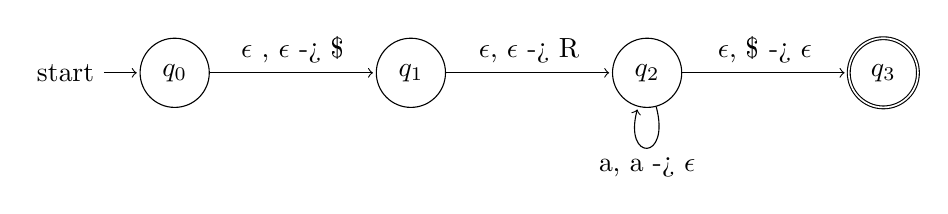
\begin{tikzpicture}[shorten >=1pt,node distance=3cm,on grid,auto] 
   \node[state,initial] (q_0)   {$q_0$}; 
   \node[state] (q_1) [right=of q_0] {$q_1$}; 
   \node[state] (q_2) [right=of q_1] {$q_2$}; 
   \node[state,accepting](q_3) [right=of q_2] {$q_3$};
    \path[->] 
    (q_0) edge  node {$\epsilon$ , $\epsilon$ -> \$} (q_1)
    (q_1) edge  node {$\epsilon$, $\epsilon$ -> R} (q_2)
    (q_2) edge  node {$\epsilon $, \$ -> $ \epsilon $} (q_3) 
          edge [loop below] node {
          a, a -> $\epsilon$} (); 
\end{tikzpicture}


\section{22 march }
\subsection{assignment 2}
We can reconnize that it is two regular languages, and that when we concatinate them we get a reglang\\
sigma star is regular, \\
we can apply theom 1.49 regular langs are closed under concat.\\
\subsection{assignemnt 3}


d)\\
	use p from pumping lemma \\
    $(xy)^{3p}(x)^p$ \\
     q

\subsection{assignemnt 5}
a)
	prove by counter exsample
    \\
    ${a^ib^ic^i | i \geq 0} \cup {a,b,c}^* $
b)
	prove by counter exsample
	${a^ib^ic^i | i \geq 0} \cup {\emptyset}$
    
    


\section{10th of April}
\begin{itemize}
\item Polynomial time reductions
\item NP-completeness
\item Examples of proofs
\begin{itemize}
\item 3-SAT
\item CLIQUE
\item Vertex cover
\item Independent set
\end{itemize}
\end{itemize}


\newpage
\section{12th of April}
\subsection{CNE-SAT is NP-Complete}
\subsubsection{Cook-lenin thm}
SAT is NP-Complete\\
 	Show that:\\
    \begin{equation}
    \forall A \in NP : A \leq_p SAT,
    \end{equation}
$ A \in NP $, Let N be a polytime NTM which accepts it in time $d_1n^k +d_2$ \\
\begin{equation}
N = (Q,\sum,R, \alpha, q_o, q_accept, q_reject).
\end{equation}
Let $W = W_1W_z*W_n$ be input to A,\\
Crate (in  polytime) a boolean formula F which is satisfiable if W is accepted by N,\\
Look at accepting breach of computation tree\\
Look at sequence of configurations.
    
\subsection{Subset-sum is NP-Complete}
   
\section{17th of April}
Hamiltonian circuit is NP-complete
\\
Conclusion on NP-complete
\\
Information on theoretic lower bound technique.

\section{1st of may}
    Approximation algorithms
    \\
    $\delta$-TSP has 2-approximation algs
    \\
    For general TSP and a fixed P, $\Delta $an alg with approx p
    \\
    Vertex cover has a 2-approx alg.
    
